\section{UAV dynamics}
\label{chap:uav_dynamics}

Modeling a system dynamics is an important part of the control design process. Good understanding of system's behavior enables to design a proper controller using approaches studied in the field of control theory. Such controller can reflect known characteristics of the system and can appropriately response to evolution of system states. There are two fundamental approaches to the system modeling. One is based on the knowledge about the physics involved in the system. This knowledge can be used to derive a mathematical model using e.g. Hamiltonian mechanics. Control design of a well known system is usually called Whitebox, or Greybox, depending on how much of the physical process we are able to describe. On the other hand, if the system is unknown, one can experimentally identify a mathematical model which sufficiently represents observed behavior of the system. Such method is usually called Blackbox.

If modeling a classical helicopter with main and tail rotors, a complex model including phenomena as aerodynamics and rotor-blade flapping could be constructed. In many approaches~\citep{alexis2014rmpc, mahony2012multirotor}, dynamics of a multirotor UAV is simplified to a single rigid-body description, mostly because of smaller fixed-pitch propellers. Further, due to existence of well designed and tested platforms such as Pixhawk~\citep{pixhawk} or Ardupilot~\citep{ardupilot}, the vehicle can be modeled with the inner feedback loop already closed. By doing that, considering a fixed-pitch quadrotor, we move from a system actuated by thrust of its four propellers to a system, where the inputs are the desired pitch ($\theta_D$), roll ($\psi_D$), yaw rate ($\dot{\phi}_D$) and collective thrust ($U_D$). It is assumed that such system can be treated as a decoupled one~\citep{mahony2012multirotor}. Some assumptions and simplifications are made in the following chapter thus the field of modeling in this thesis is the Greybox.

%Following chapter shows how the UAV's dynamics can me modeled based on the Newton's 2nd law of motion

\begin{figure}[!h]
\centering
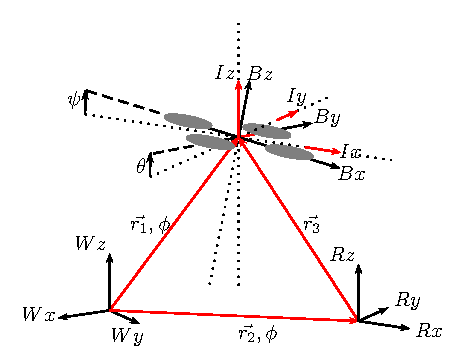
\includegraphics[width=0.7\textwidth]{fig/coordinate_system.pdf}
\caption{UAV and its coordinate systems}
\label{fig:coordinate_system}
\end{figure}

\subsection{Attitude dynamics}

Several coordinate systems are presented, in which states of the UAV~(fig.~\ref{fig:coordinate_system}) are expressed. The first one is a world coordinate system \textit{W} with a fixed position in the world. Then there is a rotating world coordinate system \textit{R}. It is rotated from $W$ around axis $W_z$ by angle $\phi$. An inertial frame \textit{I} follows, in which the attitude angles $\theta$ and $\psi$ are measured. It is translated into the geometric center of the UAV. The last one is a body frame \textit{B} which axis are aligned with the mechanical frame of the UAV.

Assuming a complete decoupling of the system, the attitude dynamics can be modeled using Newton's 2nd law of motion and expressed by following equations

\begin{equation}
\begin{split}
\ddot{x}^{(W)} &= \frac{U}{m}\left(\sin\psi\cos\phi + \sin\theta\sin\phi\right),\\
\ddot{y}^{(W)} &= \frac{U}{m}\left(\sin\theta\cos\phi + \sin\psi\sin\phi\right),\\
\end{split}
\end{equation}
\\
where $U$ is the total thrust force action on a center of gravity\footnote{in a direction of the $B_z$ axis} and $m$ is the mass of the UAV. It is assumed that desired operating point is a hovering state, where $U$, $m$ are constants and absolute values of $\theta$, $\psi$ are small. Since our system is not localized using any global localization system and it relies completely on a dead-reckoning in terms of stabilizing the yaw motion\footnote{The yaw angle $\phi$ is stabilized by a feedback loop implemented on a stabilization board using onboard IMU.}, all positions and their derivatives in following equations are expressed in system $R$. Thus the position is no longer a function of $\phi$. We can then simplify the equations into the following form

\begin{equation}
\begin{split}
\ddot{x}^{(R)} &= K_1\sin \psi,\\
\ddot{y}^{(R)} &= K_1\sin \theta.\\
\end{split}
\label{eq:attitude_first_lin}
\end{equation}

Furthermore, assuming a small input actions during hovering around the operating point, these forms can be linearized. It is done by approximating it by first two terms of the Taylor series. The acceleration of the UAV is directly proportional to its attitude angle providing assumptions previously mentioned in this paragraph. The linearized forms follows as:

\begin{equation}
\begin{split}
\ddot{x} &= K_1 \psi,\\
\ddot{y} &= K_1 \theta.\\
\end{split}
\end{equation}

\subsection{Altitude dynamics}

The altitude dynamics can be also modeled using Newton's 2nd law of motion. The following equation describes the relationship between UAV acceleration in the $R_z$ axis and control inputs $U$, $\theta$, $\psi$:

\begin{equation}
\begin{split}
\ddot{z} &= \frac{U}{m}\cos\theta\cos\psi - g^{(W)}.
\end{split}
\end{equation}

The gravitational acceleration is denoted by $g^{(W)}$. This system is also non-linear as in the case of attitude dynamics, but we need to be more cautious with a potential linearization in this case. If we try to build an altitude controller that is supposed to work not only around a hovering point, but also during take-off and landing, the force $U$ cannot be treated as constant, unlike in eq.~(\ref{eq:attitude_first_lin}). The pull force of a propeller can be simplified to a quadratic function of its angular speed \citep{luukkonen2011modelling}, which is one of the controlled inputs.

\subsection{Dynamics of the integrated stabilization}

Current UAVs are usually equipped with an attitude stabilization system. If properly tuned and the feedback loop is closed it transforms the system to be controlled by $\theta_D$, $\psi_D$, $U_D$, $\dot{\phi_D}$, instead of desired thrust of each motor. Such system can be a cheap and affordable item on a list when building a custom multirotor aircraft. For purpose of this thesis, all four model systems are modeled using first order transfer function (\ref{eq:first_order_stab}). Furthermore it is shown (chapter~\ref{cap:system_identification}) that these models are satisfactory and can be fitted on a measured data reliably. It is assumed the stabilization does not integrate an altitude feedback loop\footnote{Which would require e.g. barometer, GPS, or other sensors.}. In that case, the first order system would encapsulate also one of system integrators ($\ddot{z} \rightarrow \dot{z}$) considering an altitude speed controller, which is common in some systems \citep{pixhawk, ardupilot}. The first order transfer functions are defined as:

\begin{equation}
\begin{split}
\frac{\mathcal{L}\left\lbrace U \right\rbrace}{\mathcal{L}\left\lbrace U_D \right\rbrace} = \frac{1}{\tau_1 s + 1},\\
\frac{\mathcal{L}\left\lbrace \theta \right\rbrace}{\mathcal{L}\left\lbrace \theta_D \right\rbrace} = \frac{1}{\tau_2 s + 1},\\
\frac{\mathcal{L}\left\lbrace \psi \right\rbrace}{\mathcal{L}\left\lbrace \psi_D \right\rbrace} = \frac{1}{\tau_3 s + 1},\\
\frac{\mathcal{L}\left\lbrace \dot{\phi} \right\rbrace}{\mathcal{L}\left\lbrace \dot{\phi}_D \right\rbrace} = \frac{1}{\tau_4 s + 1}.\\
\end{split}
\label{eq:first_order_stab}
\end{equation}

\subsection{State space representation}

For the purpose of this thesis the discrete formulation of the dynamical system will be used. It allows to design a proper filtration method and the MPC controller itself. Since now, all differential equations and state space formulation are written in a discrete form with a constant sampling rate $1/\Delta t$. The following form describes a discrete time-invariant system with a main matrix $\mathbf{A}$, and input matrix $\mathbf{B}$:

\begin{equation}
\mathbf{q}_{[t+1]} = \mathbf{A}\mathbf{q}_{[t]}+ \mathbf{B}\mathbf{u}_{[t]},
\label{eq:lti_state_space}
\end{equation}
\\
where $\mathbf{x}_{t}$ is the state vector in the sample time $t$. Following matrices describe the pitch and roll systems, where state vectors are defined as $\mathbf{q}_{x} = \left(x, \dot{x}, \ddot{x}\right)^T$, $\mathbf{q}_{y} = \left(y, \dot{y}, \ddot{y}\right)^T$ and inputs as $\mathbf{u}_x = \psi_D$, $\mathbf{u}_y = \theta_D$:

\begin{equation}
\begin{split}
\mathbf{A}_{x, y} = \begin{bmatrix}
1 & \Delta t & 0 \\
0 & 1 & \Delta t \\
0 & 0 & P_1
\end{bmatrix}, \mathbf{B}_{x, y} = \begin{bmatrix}
0\\
0\\
P_2
\end{bmatrix},
\end{split}
\label{eq:attitude_LTI}
\end{equation}
\\
where $\Delta t$ is the sampling period, $P_1$ and $P_2$ are parameters of the first order transfer from a desired angle to the actual angle of attitude. This description is LTI system and can be directly used for state estimation (using e.g. Kalman filter) and for the MPC controller. For purpose of modeling altitude dynamics including Earth's gravitational pull, an additional input needs to be added to the system which will act as an constant source of acceleration. In the following case, the 2nd input value is always equal to $1$. Eq. (\ref{eq:altitude_LTI}) shows the discrete altitude LTI system for state vector $\mathbf{q}_{z} = \left(z, \dot{z}, \ddot{z}, \ddot{z}_u\right)^T$ and input $\mathbf{u}_z = \left(U_D, 1\right)^T$ linearized around a hovering point

\begin{equation}
\begin{split}
\mathbf{A}_{z} = \begin{bmatrix}
1 & \Delta t & 0 & 0\\
0 & 1 & \Delta t & 0\\
0 & 0 & 0 & 1 \\
0 & 0 & 0 & P_3
\end{bmatrix}, \mathbf{B}_{z} = \begin{bmatrix}
0 & 0\\
0 & 0\\
0 & -g\\
P_4 & 0
\end{bmatrix},
\end{split}
\label{eq:altitude_LTI}
\end{equation}
\\
where $g \approx 9.8 ms^{-2}$ is a gravitational acceleration, $P_3$ and $P_4$ are parameters of the first order system $U_D \rightarrow \ddot{z}$. The last system represents the yaw dynamics of the UAV for state vector $\mathbf{q}_{\phi} = \left(\phi, \dot{\phi}\right)^T$ and input $\mathbf{u}_\phi = \dot{\phi}_D$. Symbols $P_5$ and $P_6$ denote parameters of the system $\dot{\phi}_D \rightarrow \dot{\phi}$. The system matrices follows as:

\begin{equation}
\begin{split}
\mathbf{A}_{\phi} = \begin{bmatrix}
1 & \Delta t\\
0 & P_5 \\
\end{bmatrix}, \mathbf{B}_{\phi} = \begin{bmatrix}
0\\
P_6
\end{bmatrix}.
\end{split}
\end{equation}